\documentclass[conference]{IEEEtran}
\usepackage[utf8]{inputenc}
\usepackage{amsmath,amssymb,amsfonts}
\usepackage{graphicx}
\usepackage{cite}
\usepackage{hyperref}
\usepackage{float}
\usepackage{listings}
\usepackage{xcolor}
\usepackage{balance}

\lstset{
  basicstyle=\ttfamily\footnotesize,
  breaklines=true,
  frame=single,
  columns=fullflexible,
  backgroundcolor=\color{gray!10},
  captionpos=b
}

\title{Early Classification of Landing Quality Using Time-Series Flight Data and Gradient Boosting}

\author{\IEEEauthorblockN{Nathan Johnson}
\IEEEauthorblockA{\textit{Embry-Riddle Aeronautical University} \\
Prescott, Arizona, USA \\
johnsn63@my.erau.edu}}

\begin{document}

\maketitle

\begin{abstract}
This research presents a machine learning approach for classifying the quality of aircraft landings using time-series flight data. Utilizing flight logs from Cessna 172 aircraft equipped with Garmin G1000 avionics, a gradient boosting classifier was trained to distinguish between good and bad landings based on the final 60 seconds of flight. A custom landing detection algorithm was developed to extract and label approach segments, and features such as GPS altitude and altitude rate proved most effective for classification. The model achieved a classification accuracy of 96–99\% using 5-fold cross-validation. Attempts to forecast landing quality 20 seconds before touchdown showed a significant drop in performance, highlighting the critical importance of the final moments of flight. These results suggest strong potential for machine learning-based post-landing evaluation systems, though real-time prediction remains challenging.
\end{abstract}

\begin{IEEEkeywords}
Aviation safety, machine learning, gradient boosting, landing prediction, time-series classification
\end{IEEEkeywords}

\section{Introduction}
Landing is one of the most critical phases of flight, and poor landings can cause damage to aircraft or pose a risk to safety. In flight training environments, post-flight evaluations of landing performance are typically conducted manually by instructors. This project explores the potential for automating that process using machine learning. Specifically, I aim to develop a model capable of evaluating the final seconds of an approach and determining whether the landing is likely to be classified as "good" or "bad."

The motivation behind this work is to assist pilots—particularly students—with immediate, objective feedback and potentially inform future aircraft maintenance or safety assessments. This type of automated classification could support a range of aviation stakeholders, including flight schools, safety inspectors, and avionics developers.

This paper outlines the process of collecting, labeling, and vectorizing real-world flight data, followed by the development and training of a gradient boosting model to classify landings. I also investigate the feasibility of early classification—predicting landing quality prior to touchdown—and discuss the limitations and future directions for this line of research.

\section{Related Work}
As a pilot, I have insights into parameters influencing landing quality. Previous work, such as the 2021 study on commercial flight landings \cite{gil2022epilots}, provides valuable methodologies that can be adapted for general aviation. While that study focused on commercial aircraft, many principles, such as analyzing descent profiles, airspeed trends, and flare techniques, are applicable to this project.

\section{Dataset}
My data for this work was sourced from the flight logs created by the Garmin G1000 avionics system installed in Embry-Riddle's fleet of Cessna 172 training aircraft. I acquired logs from 396 full flights at Prescott, Arizona's municipal airport (KPRC). The raw logs were in a time-series format with one-second intervals. Features include nearly all relevant aircraft data, from barometric and GPS altitude to engine power and electrical system voltage. The flights vary in length and include diverse training activities such as pattern work (repeated landings), high-altitude maneuvers (e.g., stalls), ground reference exercises, and instrument procedures.

\section{Preprocessing}
The first step toward making this varied data usable for machine learning was to create a method for identifying landings. This was done by locating all local minima of altitude throughout the flight. To reduce noise, I required a minimum to be the lowest value within a 150-second window. Additional logic required that the minimum be within 100 feet of Prescott’s field elevation (5045 feet), and that the aircraft had been at least 500 feet above that point within the prior 180 seconds. This process was highly effective, with only 72 out of 1014 detected landings misclassified.

\begin{figure}[H]
    \centerline{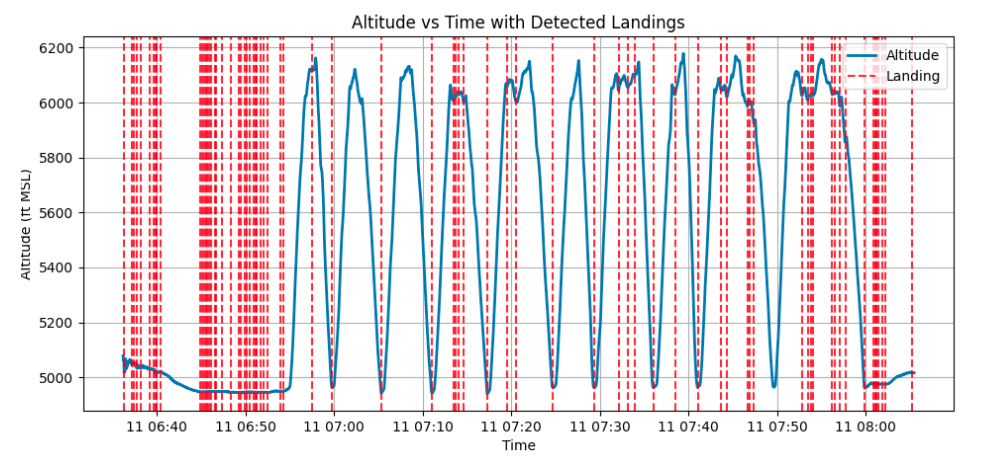
\includegraphics[width=\linewidth]{figs/local_minima_only.png}}
    \caption{Local minima only}
\end{figure}

\begin{figure}[H]
    \centerline{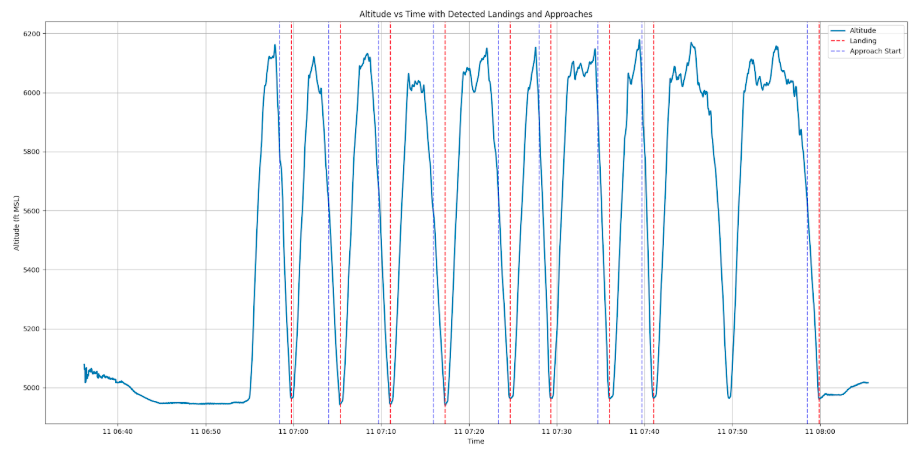
\includegraphics[width=\linewidth]{figs/additional_logic1.png}}
    \caption{Local minima with additional logic}
\end{figure}

With this detection in place, I isolated approach segments. Each approach was defined as the 60 seconds preceding a landing. This fixed-length format was essential for later vectorization. Each approach segment was saved as a separate CSV file for labeling.

\begin{figure}[H]
    \centerline{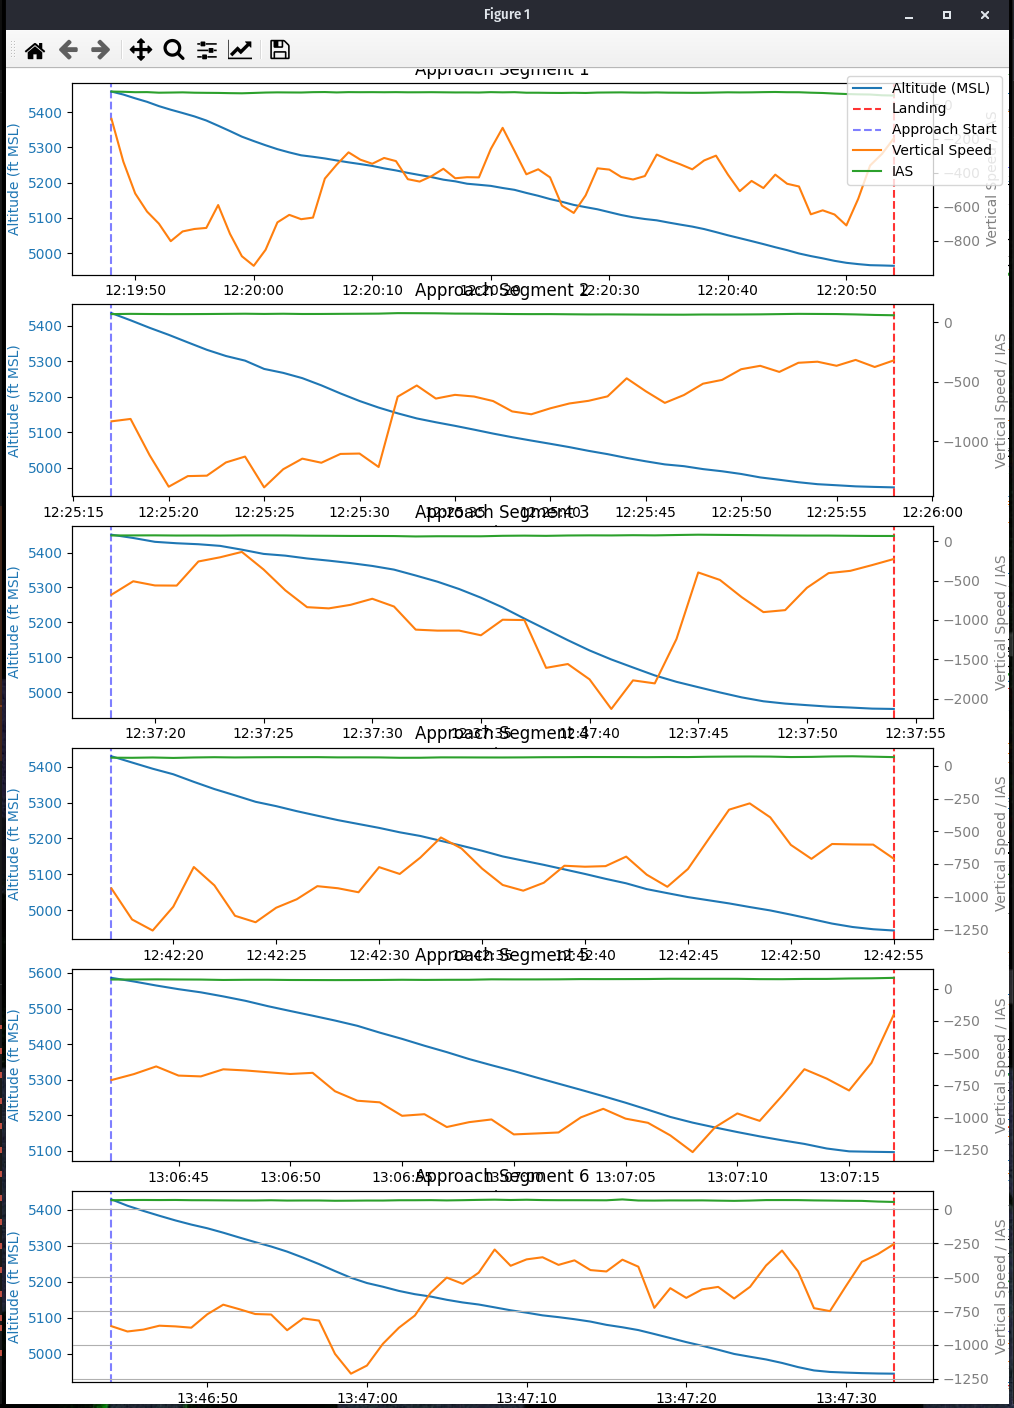
\includegraphics[width=\linewidth]{figs/approach_segments.png}}
    \caption{Isolated approach segments}
\end{figure}

Since I chose supervised learning, approaches needed to be labeled as good or bad. I manually labeled all approaches using a Python script that displayed plots of altitude and altitude rate over time. I labeled each segment as good, bad, or anomalous (e.g., false positives from the detection logic). Criteria for "bad" included a descent rate exceeding 200 feet per minute or erratic profiles without a smooth flare. Good landings featured gradual, stable descents ending in a clear flare.

\begin{figure}[H]
    \centerline{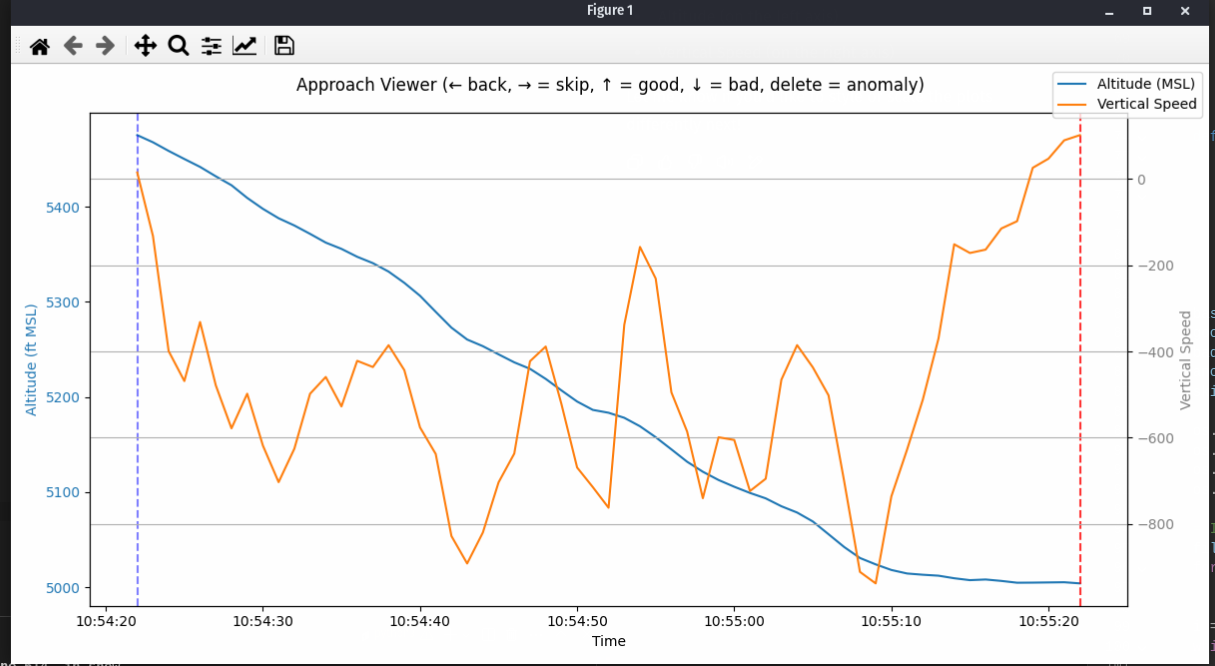
\includegraphics[width=\linewidth]{figs/approach_viewer.png}}
    \caption{Manual classification interface}
\end{figure}
  
After this labeling process, I retained 788 good and 154 bad approaches. These were vectorized by flattening each time-series into a fixed-length array: for example, a 60-second approach with altitude and altitude rate became a 120-element vector—60 values for each feature.

\section{Model Training}
I initially split the dataset into 80\% training and 20\% test data but later switched to K-fold cross-validation due to the relatively small dataset and short training times.

After testing several features—including airspeed, vertical acceleration, and engine RPM—I found that GPS altitude and altitude rate provided the best performance. This aligned with pilot intuition and significantly reduced noise from less relevant features.

I started out using a random forest model to do its relative simplicity and then switched to a gradient boosting classifier due to its potential for higher accuracy \cite{chen2016xgboost}. Using only GPS altitude and altitude rate, the model achieved excellent accuracy, with only a few misclassifications out of nearly 200 segments. Five-fold cross-validation yielded consistent results between 96\% and 99\% accuracy, suggesting a strong generalization ability and minimal overfitting.

\begin{figure}[H]
    \centerline{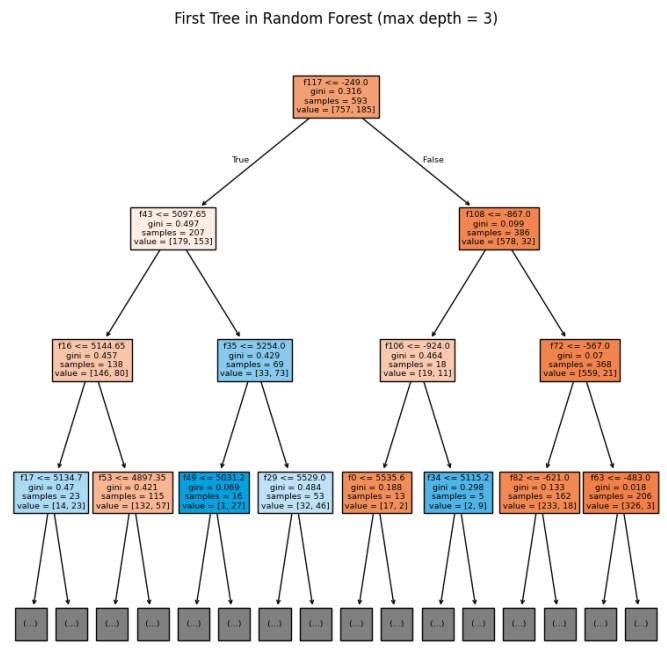
\includegraphics[width=0.6\linewidth]{figs/random_forest.png}}
    \caption{Initial random forest model}
\end{figure}

\begin{lstlisting}[caption={Initial random forest model performance}]
Cross-validation scores: [0.93650794 0.96825397 0.94148936 0.97340426 0.96276596]
Mean accuracy: 0.9564842958459978
Standard deviation: 0.01475244028636258
Confusion Matrix:
[155   3]
[  5  26]
\end{lstlisting}

\begin{figure}[H]
    \centerline{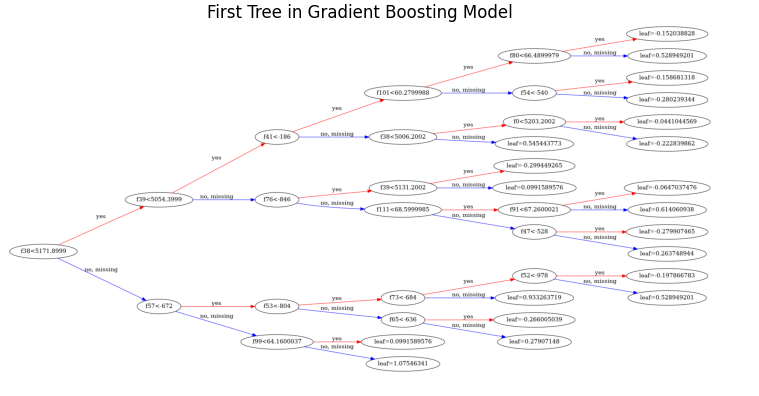
\includegraphics[width=\linewidth]{figs/gradient_boosting.png}}
    \caption{Latest gradient boosting model}
\end{figure}

\begin{lstlisting}[caption={Gradient boosting model performance}]
Cross-validation scores: [0.99470899 0.97354497 0.96276596 0.98404255 0.96276596]
Mean accuracy: 0.9755656872678149
Standard deviation: 0.012410261291420765
Confusion Matrix:
[157   1]
[  2  29]
\end{lstlisting}

To test the feasibility of early prediction, I reduced the input to only the first 40 seconds of each 60-second approach, aiming to predict landing quality 20 seconds before touchdown. However, performance dropped sharply. The model largely defaulted to classifying most landings as good, failing to identify bad landings with meaningful accuracy. In many cases, the recall for bad landings fell below 50\%.

\begin{lstlisting}[caption={Gradient boosting prediciton model performance}]
Cross-validation scores: [0.83068783 0.84656085 0.85106383 0.86170213 0.83510638]
Mean accuracy: 0.8450242035348416
Standard deviation: 0.011143484743653351
Confusion Matrix:
[152   6]
[ 25   6]
\end{lstlisting}


This suggests that many critical indicators of landing quality—such as flare execution—occur too close to touchdown to be detected earlier in the approach.

\balance

\section{Conclusion and Future Work}
Although early prediction of landing quality proved difficult, this work demonstrates that machine learning can accurately classify landings after the fact using time-series data. Such a tool could have value in flight training, maintenance diagnostics, or even post-flight briefings.

Future work could explore additional features or sensor fusion techniques, such as integrating inertial or vision-based data. While real-time prediction remains a challenge, other aspects of flight behavior could be modeled and evaluated to provide further insights into pilot performance or aircraft handling.

All of the code for this project is available at: https://github.com/nJohnson02/flight-data

\bibliographystyle{IEEEtran}
\bibliography{references}

\end{document}
